\documentclass[a4paper,12pt,twoside]{article}
\usepackage[polish]{babel}

\addto\captionspolish{\renewcommand{\figurename}{Rys.}}
\usepackage[utf8]{inputenc}
\usepackage[english]{babel}
\usepackage[margin=2cm]{geometry}
\usepackage[table,xcdraw]{xcolor}
\usepackage{graphicx}
\usepackage{indentfirst}
\usepackage{multicol}
\usepackage{listings}
\usepackage[T1]{fontenc}
\usepackage{bigfoot} % to allow verbatim in footnote
\usepackage[numbered,framed]{matlab-prettifier}
\usepackage{filecontents}
\usepackage{blindtext}
\usepackage{graphics}
\usepackage{adjustbox}
\usepackage{float}
\usepackage{subfigure}
\usepackage{multirow}
\usepackage{colortbl}
\usepackage{anyfontsize}
\usepackage{t1enc}
\usepackage{enumitem}
\usepackage{hhline}
\usepackage{fancyhdr}
\usepackage{marginnote}
\usepackage{amsmath}
\usepackage{amsthm}
\usepackage{mathtools}
\usepackage{dirtytalk}
\usepackage{cite}
\usepackage[font=footnotesize, labelfont=bf]{caption}
\usepackage{textgreek} %for units like micro in text
\usepackage[hidelinks]{hyperref}
\usepackage{adjustbox}
\urlstyle{same}
\usepackage{physics}
\usepackage{chemfig}
\renewcommand{\figurename}{Rys.}
\title{\textbf{Projekt 5: Całkowanie metodą warstwową.}}
\author{Kacper Połuszejko, 412183}
\date{}
\begin{document}
\maketitle

\section*{Wstęp}

Oszacowano wartości trzech poniższych całek za pomocą metody MC:


\[
C_1 = \int_{-3}^{3} \left(1 + \tanh(x)\right) dx = 6
\]

\[
C_2 = \int_{0}^{10} \frac{1}{1 + x^2} dx = \arctan(10) - \arctan(0)
\]

\[
C_3 = \int_{0}^{1} \cos^{10}(\pi x) dx = 0.24609375
\]


każdą za pomocą trzech metod: 1) metody podstawowej, 2) metody systematycznej, 3) metody warstwowej.

\section{Metodyka}

\subsection{Metoda podstawowa}


Dla całki postaci
\[
C = \int_a^b g(x) dx
\]

identyfikujemy fgp jako \( f(x) = \text{const} \), z warunku normalizacji dostajemy
\[
\int_a^b f(x) dx = \text{const} \int_a^b 1 dx = \text{const}(b - a) = 1 \quad \Rightarrow \quad f(x) = \frac{1}{b - a}
\]

Modyfikujemy całkę
\[
C = \int_a^b \frac{g(x)}{f(x)} f(x) dx = \int_a^b [(b - a) g(x)] f(x)
\]

a jej wartość przybliżamy średnią z próby
\[
C \approx \bar{g} = \frac{1}{N} \sum_{i=1}^N (b - a) \cdot g(x_i), \quad x_i \sim U(a, b)
\]

gdzie losowanie z rozkładu jednostajnego w zakresie \([a, b]\), wykonujemy stosując prostą transformację \( x_i = a + (b - a) \cdot U_i, \quad U_i \sim U(0, 1) \). \( U(0, 1) \) to generator liczb pseudolosowych o rozkładzie jednostajnym w przedziale \((0, 1)\). Liczymy jeszcze drugi moment

\[
\overline{g^2} = \frac{1}{N} \sum_{i=1}^N [(b - a) \cdot g(x_i)]^2 , \quad x_i \sim U(a, b)
\]

i wariancję średniej

\[
\sigma^2_{\bar{g}} = \frac{\overline{g^2} - \bar{g}^2}{N}
\]

\subsection{Metoda systematyczna}


Najpierw dokonujemy podziału obszaru całkowania na $M$ podobszarów. Załóżmy, że mają identyczną szerokość $\Delta x = (b - a)/M$. Wówczas lewą ($x_m$) i prawą ($x_{m+1}$) granicę przedziału wyznaczają
\[
x_m = a + \Delta x \cdot (m - 1), \quad m = 1, 2, \ldots, M
\]
\[
x_{m+1} = x_m + \Delta x
\]

W metodzie losowania systematycznego (warstwowego nieoptymalnego) określamy prawdopodobieństwo wylosowania zmiennej z danego podprzedziału $p_m$
\[
p_m = \int_{x_m}^{x_{m+1}} f(x) dx
\]

co dla \textbf{równomiernego podziału i jednorodnego rozkładu fgp} daje $p_m = 1/M$. Dla każdego podprzedziału $m$-tego określamy liczbę losowań
\[
N_m = p_m \cdot N
\]

obliczamy $n = 1$ i $2$ moment oraz wariancję
\[
\overline{g^n}_m = \frac{1}{N_m} \sum_{i=1}^{N_m} [(b - a) \cdot g(x_{im})]^n, \quad x_{im} \sim U(x_m, x_{m+1})
\]
\[
\sigma^2_m = \overline{g^2}_m - (\overline{g}_m)^2
\]

Teraz możemy oszacować wartość całki $C$ jako średnią i wariancję średniej
\[
C \approx \bar{g} = \sum_{m=1}^M p_m \cdot \bar{g}_m
\]
\[
\sigma^2_{\bar{g}} = \sum_{m=1}^M \frac{p_m^2}{N_m} \cdot \sigma^2_m
\]

\subsection{Metoda warstwowa}

W metodzie tej postępujemy identycznie jak dla losowania systematycznego poza jednym wyjątkiem, liczbę losowań $N_m$ w każdym podprzedziale określamy według wzoru
\[
N_m = \frac{p_m \hat{\sigma}_m}{\sum_{j=1}^M p_j \hat{\sigma}_j} \cdot N
\]

gdzie: $\hat{\sigma}_j$ to prognozowane/szacowane wartości odchylenia standardowego, które obliczamy metodą systematyczną dla małej wartości $N$ (np. $N = 10^2, 10^3$) — bo dokładnych wartości nie znamy. Oczywiście w trakcie wykonywania właściwych obliczeń (metoda warstwowa) na bieżąco wyznaczamy „dokładniejsze” wartości $\sigma_m$ i ich ostatecznie używamy do liczenia wariancji średniej.

\section{Wyniki}


\begin{enumerate}
    \item Zaimplementowano podstawową metodę Monte Carlo do całkowania w celu oszacowania wartości całki $C_1$. Dla kolejnych wartości $N = 10^k$, gdzie $k = 2, 3, 4, 5$, obliczono wartość całki, odchylenie standardowe średniej $\sigma_{\bar{g}}$ oraz względny błąd $R = \frac{\sigma_{\bar{g}}}{\bar{g}} \cdot 100\%$. Przedział $[a, b]$ podzielono na $M = 10$ równych podprzedziałów. Dla każdego $N$ określono liczbę losowań przypadających na każdy z podprzedziałów i stworzono odpowiednie histogramy. Wyniki zestawiono w tabeli.

    \item Zaimplementowano metodę losowania systematycznego i powtórzono obliczenia wykonane w punkcie 1.

    \item Zaimplementowano metodę losowania warstwowego i ponownie wykonano obliczenia z punktu 1. Dodatkowo, oszacowano wartość $\hat{\sigma}_m$ przy użyciu metody systematycznej, wykonując 100 losowań (dla metody warstwowej przy $N = 10^2$) oraz 1000 losowań (dla metody systematycznej przy $N > 10^3$). 

    \item Obliczenia z punktów 1–3 powtórzono dla całek $C_2$ oraz $C_3$.

    \item Wyniki przedstawiono w formie tabel. Dodatkowo zamieszczono przykładowe histogramy rozkładu liczby losowań.
\end{enumerate}

\vspace{8mm}

\textbf{Tabela 1} Oszacowane wartości całek $C_1, C_2, C_3$ oraz ich odchylenia standardowe średniej i błędy względne.
\begin{table}[h!]
\centering
\begin{minipage}[t]{0.32\textwidth}
\centering
\caption*{$C_1$}
\hspace{-6mm}
\begin{tabular}{|c|c|c|c|}
\hline
\multicolumn{4}{|c|}{Metoda podstawowa} \\ \hline
N & $\bar{g}$ & $\sigma_{\bar{g}}$ & R [\%] \\ \hline
$10^2$ & 5.776 & 0.481 & 8.341 \\ \hline
$10^3$ & 6.206 & 0.153 & 0.024 \\ \hline
$10^4$ & 5.980 & 0.0490 & 0.821 \\ \hline
$10^5$ & 6.013 & 0.0155 & 0.259 \\ \hline
\multicolumn{4}{|c|}{Metoda systematyczna} \\ \hline
$10^2$ & 6.109 & 0.0398 & 0.650 \\ \hline
$10^3$ & 5.985 & 0.0154 & 0.258 \\ \hline
$10^4$ & 6.002 & 0.0049 & 0.081 \\ \hline
$10^5$ & 6.001 & 0.00151 & 0.026 \\ \hline
\multicolumn{4}{|c|}{Metoda warstwowa} \\ \hline
$10^2$ & 6.030 & 0.0367 & 0.608 \\ \hline
$10^3$ & 6.003 & 0.0108 & 0.180 \\ \hline
$10^4$ & 5.996 & 0.0034 & 0.057 \\ \hline
$10^5$ & 6.0002 & 0.0011 & 0.018 \\ \hline
\end{tabular}
\end{minipage}
\hfill
\begin{minipage}[t]{0.32\textwidth}
\centering
\caption*{$C_2$}
\begin{tabular}{|c|c|c|c|}
\hline
\multicolumn{4}{|c|}{Metoda podstawowa} \\ \hline
N & $\bar{g}$ & $\sigma_{\bar{g}}$ & R [\%] \\ \hline
$10^2$ & 1.076 & 0.193 & 17.969 \\ \hline
$10^3$ & 1.499 & 0.0751 & 5.011 \\ \hline
$10^4$ & 1.481 & 0.0241 & 1.619 \\ \hline
$10^5$ & 1.478 & 0.0075 & 0.511 \\ \hline
\multicolumn{4}{|c|}{Metoda systematyczna} \\ \hline
$10^2$ & 1.525 & 0.0568 & 3.725 \\ \hline
$10^3$ & 1.470 & 0.0179 & 1.216 \\ \hline
$10^4$ & 1.471 & 0.0058 & 0.396 \\ \hline
$10^5$ & 1.468 & 0.0019 & 0.127 \\ \hline
\multicolumn{4}{|c|}{Metoda warstwowa} \\ \hline
$10^2$ & 1.462 & 0.0260 & 1.780 \\ \hline
$10^3$ & 1.546 & 0.0551 & 3.566 \\ \hline
$10^4$ & 1.486 & 0.0240 & 1.613 \\ \hline
$10^5$ & 1.467 & 0.0067 & 0.456 \\ \hline
\end{tabular}
\end{minipage}
\hfill
\begin{minipage}[t]{0.32\textwidth}
\centering
\caption*{$C_3$}
\begin{tabular}{|c|c|c|c|}
\hline
\multicolumn{4}{|c|}{Metoda podstawowa} \\ \hline
N & $\bar{g}$ & $\sigma_{\bar{g}}$ & R [\%] \\ \hline
$10^2$ & 0.316 & 0.0372 & 11.793 \\ \hline
$10^3$ & 0.229 & 0.0105 & 4.564 \\ \hline
$10^4$ & 0.246 & 0.0034 & 1.381 \\ \hline
$10^5$ & 0.247 & 0.0011 & 0.435 \\ \hline
\multicolumn{4}{|c|}{Metoda systematyczna} \\ \hline
$10^2$ & 0.253 & 0.0072 & 2.845 \\ \hline
$10^3$ & 0.247 & 0.0028 & 1.137 \\ \hline
$10^4$ & 0.246 & 0.0008 & 0.344 \\ \hline
$10^5$ & 0.246 & 0.0003 & 0.114 \\ \hline
\multicolumn{4}{|c|}{Metoda warstwowa} \\ \hline
$10^2$ & 0.243 & 0.0144 & 5.911 \\ \hline
$10^3$ & 0.228 & 0.0087 & 3.803 \\ \hline
$10^4$ & 0.244 & 0.0029 & 1.194 \\ \hline
$10^5$ & 0.247 & 0.0009 & 0.344 \\ \hline
\end{tabular}
\end{minipage}
\end{table}

Na podstawie powyższej tabeli można stwierdzić, że metoda podstawowa radzi sobie zdecydowanie najgorzej dla każdej z szacowanych całek. Metoda warstwowa daje najlepsze wyniki dla całki $C_1$, natomiast metoda systematyczna dla całek $C_2$ i $C_3$.

\newpage
\begin{figure}[h!]
\hspace{-10mm}
    \begin{minipage}{0.55\textwidth}
        \centering
        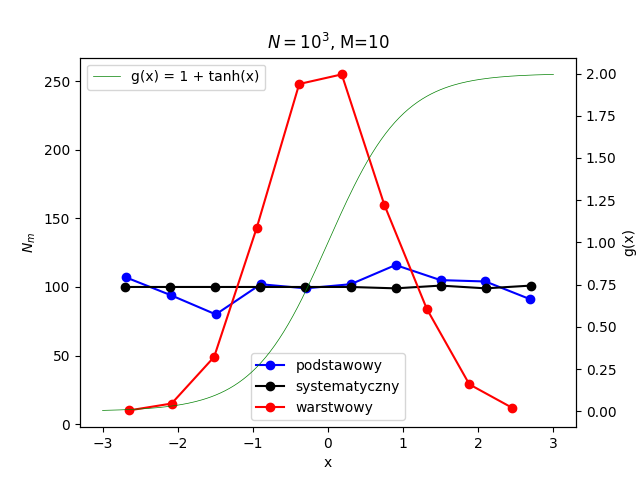
\includegraphics[scale = 0.55]{histogram3.jpg}
    \end{minipage}
    %\hspace{15mm}
    \begin{minipage}{0.55\textwidth}
        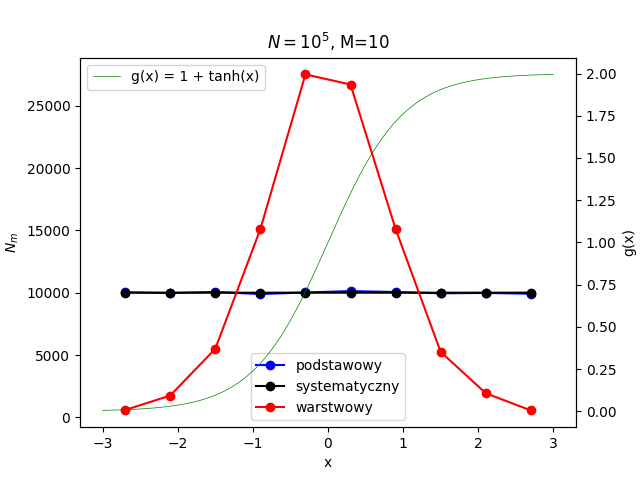
\includegraphics[scale = 0.55]{histogram5.png}
    \end{minipage}
    \caption{Histogramy rozkładu ilości losowań dla całki $C_1$. Po lewej dla $N = 10^3$, po prawej dla $N = 10^5$.}
\end{figure}

Jak widać na powyższych wykresach, w metodzie systematycznej rozkład ilości losowań jest jednorodny, co jest oczywiste, jako że liczba losowań w każdym z podprzedziałów jest identyczna, co wynika ze wzorów. W przypadku metody podstawowej wykonano $N$ losowań za pomocą rozkładu jednorodnego na całym przedziale, dlatego widocznie są drobne różnice w każdym z podprzedziałów (dla $N=10^5$, są już jednak znacznie mniejsze). Natomiast w przypadku metody warstwowej liczba losowań rośnie dla podprzedziałów, w których funkcja $g(x)$ najbardziej się zmienia. Dzięki temu generuje też ona najdokładniejsze wyniki, co widać w \textbf{Tabeli 1}.

\end{document}
